\documentclass[12pt]{article}
\usepackage{graphicx} % Required for inserting images
\usepackage{xcolor}
\usepackage{titlesec}
\usepackage{mdframed}
\usepackage{amsmath}
\usepackage[a4paper,left=22mm,top=20mm,right=22mm]{geometry}
\usepackage{hyperref}

\title{Calculus II - Chapter 1 \\  Function of several variables }

\author{By Minh Nguyen Quang from USTH Learning Support}
\date{April 2024}
\newmdenv[linecolor=black,skipabove=\topsep,skipbelow=\topsep,
leftmargin=-5pt,rightmargin=-5pt,
innerleftmargin=5pt,innerrightmargin=5pt]{mybox}

\begin{document}

\maketitle
\tableofcontents
\newpage
\section{The set $R^n$}
\subsection{Definition}
The set of $R^n$ consists of all n-tuples $(x_1,x_2,..x_n)$ with real entries .\\
Two operations:\\
- Addiction\\
- Scalar multiplication
\subsection{Some equations in $R^2$}

$\bullet$ Equation of a line:
$$  ax+by= c, (a^2+b^2 \neq 0) $$
$\bullet$ Equation of a circle:
$$(x-a)^2 +(y-b)^2 = r^2, (r>0)$$
$\bullet$ Equation of an ellipse:
$$\alpha(x-a)^2 + \beta(y-b)^2 = r^2 , \alpha > 0,\beta>0, r>0 $$
\subsection{Some equation in $R^3$}

$\bullet$ Equation of a plane
$$ ax + by +cz = d, a^2 +b^2 +c^2 \neq 0$$
 \paragraph{ vector n = (a,b,c) perpendicular with plane.\\}
$\bullet$ Equation of a sphere: center (a, b, c), radius r
$$(x-a)^2 +(y-b)^2 + (z-c)^2 =r^2, r >0 $$

$\bullet$ Equation of an ellipsoid:

$$\alpha(x-a)^2 +\beta(y-b)^2 + \gamma(z-c)^2 =r^2, \alpha,\beta,\gamma, r >0 $$

\section{Function of several variables}
\subsection{Definition}
 A function f of n variables with a domain D $\subset R^n$, is a rule that assigns to each point $(x_1,x_2,..,x_n)$ $\in$ D a unique number denoted by $f(x_1,x_2,..x_n)$. \\
 $\ast$ Note: \\
 - In this course, we often consider function of 2 or 3 variables. \\
 - w = $f(x_1,..,x_n)$ called dependent variable and $x_1,x_2,..$ called independent variables.\\

Example: Find domain of $f(x,y)= \frac{\sqrt{x+y+1}}{x-1}$ and evaluate $f(3,5)$ \\ 
\begin{center}
\textbf{Solution}    
\end{center}

$D = \{(x,y)|x+y+1 \geq 0 $ and $  x \neq 1$\} \\  
$f(3,5) = \frac{3}{2}$ \\
\begin{center}
    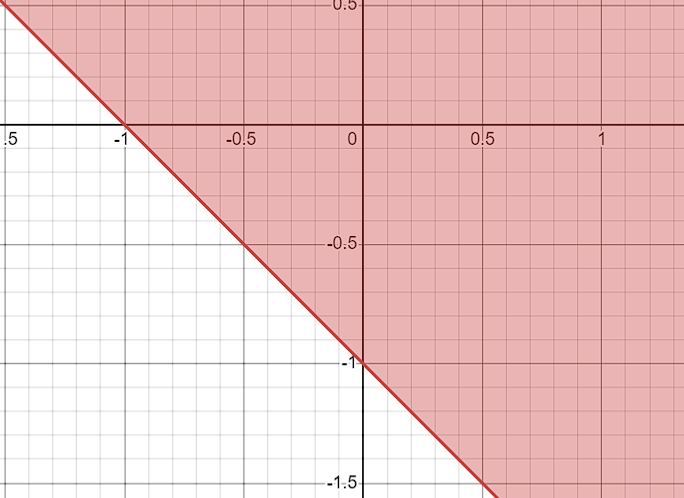
\includegraphics[scale=0.5]{domain.png}
\end{center}


\subsection{Level curve for function of 2 variables}
- The level curves of a function f of two variables are curve with equation $f(x,y)=k$, where k is a constant (in range of $f$). 

Example: Graph $f(x,y) = 100 -x^2 -y^2$ and plot the level curve $f(x,y)=0,f(x,y) = 100$.\\ 
Sol:\\
Domain : $D = \{(x,y) \in R^2$\} \\
Range: $R = \{z \in R | z \leq 100\}$\\
With $f(x,y) = 100 -x^2 -y^2 = 0$, then $x^2 +y^2 =100$ $\rightarrow$ the level curve in this case is a circle with center at (0,0) and radius = 10. \\
With $f(x,y) = 100$, then level curve in this case is origin.\\ 
\begin{center}
    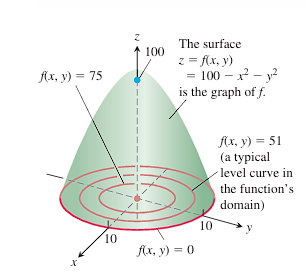
\includegraphics[scale=1]{Ảnh chụp màn hình 2024-03-26 025527.png}
\end{center}

- If $f(x, y)$ is the altitude function of a region in $R^2$
, then the level curves give rise to the contour map.\\
\begin{center}
    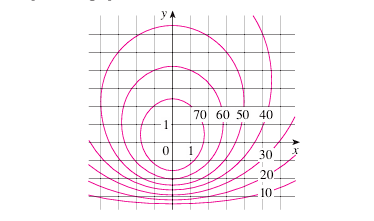
\includegraphics[scale=1]{Ảnh chụp màn hình 2024-03-26 030911.png}
\end{center}

\subsection{Level surface for function of 3 variables }
- For a function f of three variables, the set of points $(x, y, z) \in R^3$ where $f(x, y, z)$ has a constant value f(x, y, z) = k is called a level surface of f.\\
\begin{center}
    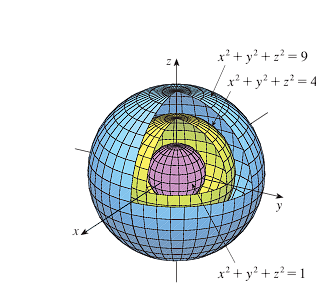
\includegraphics[scale = 1]{i.png}
\end{center}

Example: Consider function $f(x,y,z)=(x-1)^2 +(y-2)^2+ (z-3)^2$. Find the level surface which pass through point (4,5,6)\\
Sol: $f(4,5,6)=27$, so level surface which passes through point (4,5,6) is  $(x-1)^2 +(y-2)^2+ (z-3)^2=27$\\
This is a sphere centered at (1,2,3) with radius is $\sqrt{27}$
\subsection{Exercise}
1. Match function with its graph.\\
   - $z=\sin(xy)$ \\
   - $z = \sin(x-y)$ \\
   - $z = (1-x^2)(1-y^2)$\\
   -$z = \sin x - \sin y $\\
   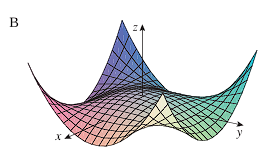
\includegraphics[scale=1]{1.png}
   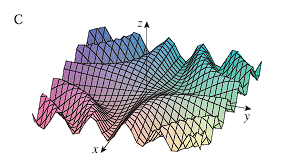
\includegraphics[scale=1]{2.png}\\
   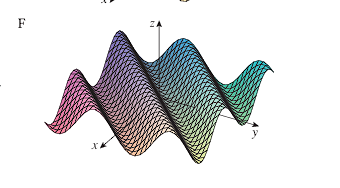
\includegraphics[scale=1]{3.png}
   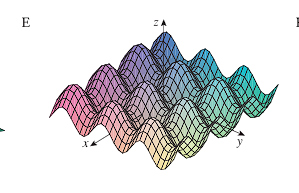
\includegraphics[scale=1]{4.png}\\
   - Hint: Based on the specific values such as x=0,y=0,.. and properties of the function.\\ 
   - Answer: \\B: $(1-x^2)(1-y^2)$\\
             C: $\sin(xy)$\\
             F: $\sin(x-y)$ \\
             E: $\sin x - \sin y $\\
\section{Limit}
\subsection{Definition}
Let $f$ be a function of two variables defined on a domain $D \subset R^2$ and $(a,b) \subset R^2$ ( (a,b) do not necessary tin D)\\
\\
We say that the limit of $f(x, y)$ as (x, y) tends to (a, b) exists, if there is a number L such that
\begin{mybox}
    For any $\varepsilon > 0$ there exist a corresponding $\delta > 0$ such that\\
    $|f(x,y) -L | <\varepsilon$ whenever $0 < ||(x,y) - (a,b) || <\delta$, $(x,y) \in D$ \\
    \\
    And we write: $$\lim_{(x,y) \to\ (a,b)} f(x,y) = L$$
    
\end{mybox} 
- If limit of a function at one point (x,y) exists, then it is unique.\\
- Can't apply L'Hospital rule to find limit in function of several variables.\\  
- The Squeeze Theorem is also true for function of several variables.\\
$\bullet Example:$ Given function $f(x,y) = \frac{xy}{\sqrt{x^2+y^2}}$, find $\lim_{(x,y) \to\ (0,0)}$?\\
\begin{center}
    \textbf{Solution}
\end{center}
D = $R^2 \setminus {(0,0)}$\\
This is indeterminate form $\frac{0}{0}.$\\ 
Consider $|\frac{xy}{\sqrt{x^2+y^2}}|$\\
We have $\sqrt{x^2} \leq \sqrt{x^2 +y^2}$, so $|\frac{xy}{\sqrt{x^2+y^2}}| \leq |\frac{xy}{\sqrt{x^2}}| = |y|$ \\
$\rightarrow$ $-|y| \leq \frac{xy}{\sqrt{x^2+y^2}} \leq |y|$\\
Using Squeeze Theorem: \\
$$\lim_{(x,y) \to \ (0,0)} -|y| \leq \lim_{(x,y) \to \ (0,0)} f(x,y) \leq \lim_{(x,y) \to \ (0,0)} |y|$$ 
$$\rightarrow \lim_{(x,y) \to \ (0,0)} f(x,y) = 0 $$\\ 

\begin{center}
    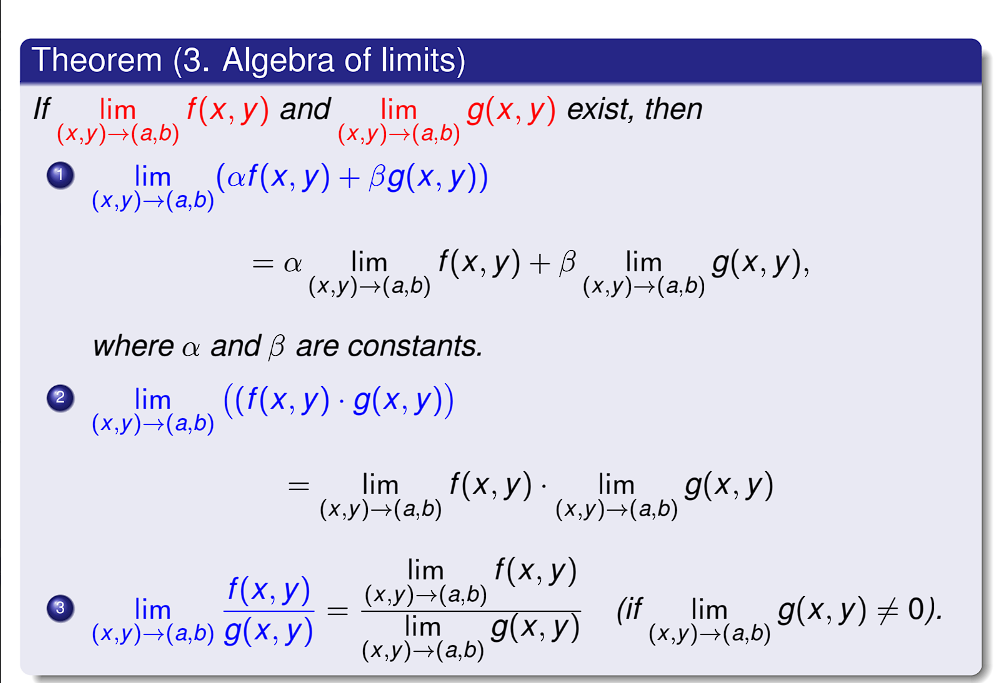
\includegraphics[scale = 0.5]{5.png}\\
\end{center}


\subsection{Limit along a path}
\begin{center}
    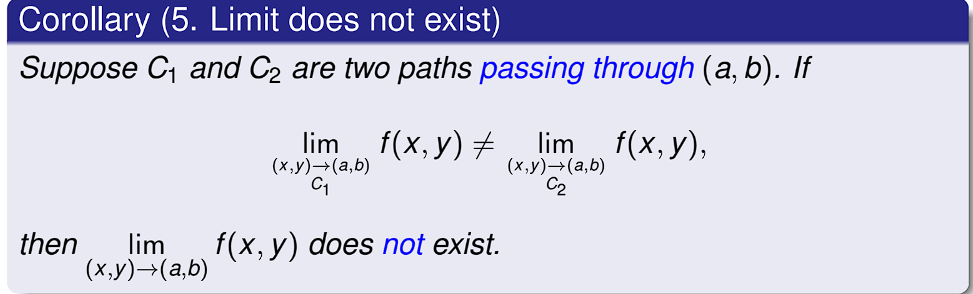
\includegraphics[scale= 0.5 ]{6.png} \\
\end{center}


$\bullet Note:$\\
- To prove the limit does not exist, you need to find two paths passing through (a,b) that make two different limit.\\
- Only use limit along a path to prove the limit does not exist. \\
\\
Example: Find limit: $\lim_{(x,y) \to \ (0,0)} \frac{xy^2}{x^2 + y^4} $

\begin{center}
    \textbf{Solution}
\end{center}
Choose first path: y = x, substitute y = x, we have:
$$\lim_{(x,y) \to \ (0,0)} \frac{xy^2}{x^2 + y^4} =  \lim_{(x,y) \to \ (0,0)} \frac{x^3}{x^2 + x^4} = 0 $$ 
Choose second path: $x = y^2$, substitute $x = y^2$, we have:
$$\lim_{(x,y) \to \ (0,0)} \frac{xy^2}{x^2 + y^4} =  \lim_{(x,y) \to \ (0,0)} \frac{y^4}{y^4 + y^4} = \frac{1}{2} $$ 
$\rightarrow$ limit does not exist 

\section{Continuity}

$f(x,y)$ is continuous at point (a,b), if satisfy 3 conditions: \\
- (a,b) $\in$ domain of $f$\\
- $\lim_{(x,y) \to \ (a,b)} f$ exists\\
- $\lim_{(x,y) \to \ (a,b)} f = f(a,b)$\\
\\
$\bullet$ Note: Polynomial and rational function are always continuous on their domain. 

 \section{Partial Derivative}
 \subsection{Definition}
 \subsubsection{Partial Derivative of Function of 2 variables}
 \begin{mybox}
    For a function of two variables $f(x,y)$, partial derivative of $f$ with respect to x is a function $f_x$ defined as follow:
    $$f_x (x,y) = \lim_{t \to \ x} \frac{f(t,y) - f(x,y)}{t-x}$$
    (keeping y as a constant)
    
\end{mybox}
 Another notation: $\frac{\partial f}{\partial x}$ (write $\frac{df}{dx}$ when calculating partial derivative = 0 points.)
 \begin{center}
     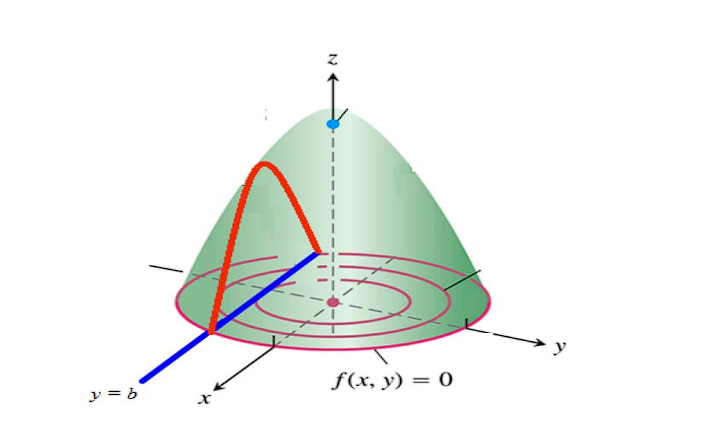
\includegraphics[scale =0.5]{7.png}
 \end{center}
 
 
(This image illustrates a partial derivative w.r.t. x and we consider the derivative on the red line.) 
\begin{mybox}
    Partial Derivative of $f$ w.r.t y defined by formula: 
  $$f_y (x,y) = \lim_{t \to \ y} \frac{f(x,t) - f(x,y)}{t-y}$$ (keep x as a constant)
  
\end{mybox}

 Example: Use the definition to calculate $f_x(x,y),f_y(x,y)$. With $f(x,y) = 4x^2y^4$   
 \begin{center}
     \textbf{Solution}
 \end{center}
$$ f_x(x,y) = \lim_{t \to\ x} \frac{4t^2y^4 - 4x^2y^4}{t-x} =\lim_{t \to\ x} \frac{4y^4(t^2-x^2)}{t-x} = \lim_{t \to\ x} \frac{4y^4(t-x)(t+x)}{t-x} = \lim_{t \to\ x} 4y^4(t+x) $$
$= 4y^42x =8xy^4$

$$ f_y(x,y) = \lim_{t \to\ y} \frac{4x^2t^4 - 4x^2y^4}{t-y} =\lim_{t \to\ y} \frac{4x^2(t^4-y^4)}{t-y} = \lim_{t \to\ y} \frac{4x^2(t^2-y^2)(t^2+y^2)}{t-y}  $$
$$= \lim_{t \to\ y} 4x^2(t^2+y^2)(t+y) = 4x^2 2y^2 2y =16x^2y^3 $$

$\bullet$ You can define partial derivative in term of $h \rightarrow 0$

1. Let t = x + h, when t $\rightarrow x$, then h $\rightarrow$ 0.\\
$$f_x(x,y) = \lim_{h\to\ 0} \frac{f(x+h,y)- f(x,y)}{h}$$
2. Let t = y+h,  when t $\rightarrow y$, then h $\rightarrow$ 0.\\
$$f_y(x,y) = \lim_{h\to\ 0} \frac{f(x,y+h)- f(x,y)}{h}$$
\subsubsection{ Partial Derivative of Function of n variables}
\begin{mybox}
    For a function of several variables $f(x_1,x_2,..,x_i...,x_n)$, partial derivative of $f$ with respect to $x_i$ is a function $f_x{}_i$ defined as follow:
  $$f_x{}_i (x_1,x_2,..,x_n) = \lim_{h \to \ 0} \frac{f(x_1,x_2,..,x_i+h,..x_n) - f(x_1,x_2,..,x_i,..x_n)}{h}$$
    
    
\end{mybox}

Another notation $\frac{\partial f}{\partial x_i}$\\
$\bullet$ To evaluate $f_x$, we regard y as a constant and differentiate
the function $f(x, y)$ with respect to x.\\
$\bullet$ To evaluate $f_y$, we regard x as a constant and differentiate
the function $f(x, y)$ with respect to y.\\

Example: Find $f_x(x,y)$ and $f_y(x,y)$, if $f(x,y) = cos(3x^2+y)y^5 $
 \begin{center}
     \textbf{Solution}
 \end{center}
 $$f_x(x,y) = -sin(3x^2+y)6xy^5$$
 $$f_y(x,y) = -sin(3x^2+y)y^5 + cos(3x^2+y)5y^4$$
 
 Example: Find $f_x(x,y,z)$,$f_z(x,y,z)$ and $f_y(x,y,z)$, if $f(x,y,z) = 3x^2y^5ln(z) $
  \begin{center}
     \textbf{Solution}
 \end{center}
 $$f_x(x,y,z) = 6xy^5ln(z)$$
 $$f_z(x,y,z)= 3x^2y^5\frac{1}{z}$$
 $$f_y(x,y,z)= 3x^25y^4ln(z)$$
 
 \subsection{Second Partial Derivative}
 $\bullet$  If is a function of two variables, then its partial derivatives and are also functions of two variables, so we can consider their partial derivatives $f_x{}_x$,$f_x{}_y$,$f_y{}_x$,and $f_y{}_y$ , which are called the second partial derivatives of $f$ . If z =$f(x,y)$ , we use the following notation:\\
 \\
 $$f_x{}_x = (f_x)_x = \frac{\partial}{\partial x} \frac{\partial f}{\partial x}= \frac{\partial^2 f}{\partial x^2}$$
 $$f_x{}_y = (f_x)_y = \frac{\partial}{\partial y} \frac{\partial f}{\partial x}= \frac{\partial^2 f}{\partial y \partial x}$$
 $$f_y{}_y = (f_y)_y = \frac{\partial}{\partial y} \frac{\partial f}{\partial y}= \frac{\partial^2 f}{\partial y^2}$$
 $$f_y{}_x = (f_y)_x = \frac{\partial}{\partial x} \frac{\partial f}{\partial y}= \frac{\partial^2 f}{\partial x \partial y}$$
 Note: Notice the order of $\partial x$, $\partial y$\\
 It is similar with function of 3 variables.\\
 \\
 Example: Find all second-order derivatives of $f(x,y) = 3x^2 + 4xy^3 + y^5$ \\
 \begin{center}
     \textbf{Solution}
 \end{center}
 $$f_x(x,y) = 6x + 4y^3$$
 $$f_y(x,y) = 12xy^2 + 5y^4$$
 $$(f_x)_x = 6$$
 $$(f_x)_y = 12y^2$$
 $$(f_y)_x = 12y^2$$
 $$(f_y)_y = 24xy + 20y^3$$
 
 \begin{mybox}
     Clairaut’s Theorem: If $f(x,y)$ and its partial derivative $f_x, f_y, f_x{}_y, f_y{}_x$ are defined throughout an open region containing a point (a, b) and all are continuous at (a, b), then:
     $$f_x{}_y = f_y{}_x$$
 \end{mybox}
 
 \subsubsection{ Gradient vector}
 Gradient vector is formed by partial derivative of f.
 \begin{mybox}
     1. For a function of two variables $f(x,y)$, gradient vector of f is a vector $\nabla f $ defined by:
     $$\nabla f = (f_x,f_y) = (\frac{\partial f}{\partial x} i,\frac{\partial f}{\partial y}j)$$
     2. For a function of three variables $f(x,y,z)$, gradient vector of f is a vector $\nabla f $ defined by:
     $$\nabla f = (f_x,f_y,f_z) = (\frac{\partial f}{\partial x} i,\frac{\partial f}{\partial y}j, \frac{\partial f}{\partial z}k)$$
     3. For a function of n variables $f(x_1,x_2,..x_n)$, gradient vector of is a vector $\nabla f $ defined by:
     $$\nabla f = (f_x{}_1,f_x{}_2,..,f_x{}_n) $$
 \end{mybox}
 Example: For function $f(x,y,z) = 3x^2 + y^3 +z^4 +4xyz$ \\
 a. Find gradient vector of $f$ \\
 b.  Find gradient vector of $f$ at point $P_o$ (1,2,3)
 \begin{center}
     \textbf{Solution}
 \end{center}
 a.
 $$f_x = 6x + 4yz$$
 $$f_y = 3y^2 + 4xz$$
 $$f_z = 4z^3 +4xy$$
 $$\nabla f = (f_x, f_y,f_z) = (6x + 4yz,3y^2 + 4xz,4z^3 +4xy)$$
 b. \\
 $$\nabla P_o = (30,24, 116)  $$
 
 \section{The chain rule}
 \subsection{The chain rule - Case 1}
 For a function $f(x, y)$, when both x and y are functions of ONE
variable.

\begin{mybox}
    If w = $f(x, y)$ is differentiable and x = x(t), y = y(t) are differentiable functions of t, then the composite function w = $f(
x(t), y(t))$ is also differentiable w.r.t. t and:
$$\frac{dw}{dt} = \frac{\partial w}{\partial x} \frac{dx}{dt}+ \frac{\partial w}{\partial y} \frac{dy}{dt}$$
\end{mybox}
 Example: Suppose $w = 6x^2+3y^4$, where x = 5t+1, $y = t^2$.Find $\frac{dw}{dt}$ 
 \begin{center}
     \textbf{Solution}
 \end{center}
 $$\frac{\partial w}{\partial x} = 12x$$
 $$\frac{dx}{dt}=5$$
 $$\frac{\partial w}{\partial y} = 12y^3$$
 $$\frac{dy}{dt} = 2t$$
 $$\frac{dw}{dt} = \frac{\partial w}{\partial x} \frac{dx}{dt}+ \frac{\partial w}{\partial y} \frac{dy}{dt} = 12x5 + 12y^32t = 60(5t+1) + 12(t^2)^3 \times 2t = 300t+24t^7+60$$
\\
 Example: The voltage V in a circuit that 
satisfies the law V=IR is slowly dropping as the battery wears 
out. At the same time, the resistance R is increasing as the resistor 
heats up. Find how the current is changing at the instant when R = 
600 ohms, I=0.04 amp, $\frac{dR}{dt}$ =0.5 ohm/sec, and $\frac{dV}{dt}$= -0.01 volt/sec.\\
Sol:\\
Using the chain rule, we have:\\
$$\frac{dV}{dt} = \frac{\partial V}{\partial I}\frac{dI}{dt} + \frac{\partial V}{\partial R}\frac{dR}{dt}$$

$$\frac{dV}{dt} = R\frac{dI}{dt} + I\frac{dR}{dt}$$
$$-0.01 = 600\frac{dI}{dt}+0.04\times0.5$$
$$\rightarrow \frac{dI}{dt} = -5\times10^{-5} amp/sec$$
\\

\begin{mybox}
    It is similar for function of n variables. If $w = f(x_1,x_2,..,x_n)$ is differentiable and $x_1 = x_1(t), x_2 =x_2(t),..,x_n = x_n(t)$ are differentiable, then w is also differentiable w.r.t t:
    $$\frac{dw}{dt}=\frac{\partial w}{\partial x_1}\frac{dx_1}{dt}+ \frac{\partial w}{\partial x_2}\frac{dx_2}{dt}+...+\frac{\partial w}{\partial x_n}\frac{dx_n}{dt} $$
\end{mybox}
\subsection{The chain rule - Case 2}
For a function f(x, y), when both x and y are functions of TWO
variables.\\
\begin{mybox}
    If $w = f(x, y)$, where $x = g(s, t)$ and $y = h(s, t)$ are differentiable, then w has partial derivatives w.r.t. s and t, and:
    $$\frac{\partial w}{\partial s} = \frac{\partial w}{\partial x}\frac{\partial x}{\partial s}+\frac{\partial w}{\partial y}\frac{\partial y}{\partial s}$$
    $$\frac{\partial w}{\partial t} = \frac{\partial w}{\partial x}\frac{\partial x}{\partial t}+\frac{\partial w}{\partial y}\frac{\partial y}{\partial t}$$
\end{mybox}
Example: For $w = 2x^2 + 3xy^2$, where x = 3t + 4z, $y = 3t^3 +z^2$. Find $\frac{\partial w}{\partial t}$, $\frac{\partial w}{\partial z}$ when t = z = 1
 \begin{center}
     \textbf{Solution}
 \end{center}
$$\frac{\partial w}{\partial x} = 4x + 3y^2 = 76 $$
$$\frac{\partial w}{\partial y} = 6xy = 168$$
$$\frac{\partial x}{\partial t}= 3$$
$$\frac{\partial x}{\partial z}= 4$$
$$\frac{\partial y}{\partial t} = 9t^2 = 9$$
$$\frac{\partial y}{\partial z}= 2z = 2$$
$$\frac{\partial w}{\partial z} = \frac{\partial w}{\partial x}\frac{\partial x}{\partial z}+\frac{\partial w}{\partial y}\frac{\partial y}{\partial z} =  640$$
$$\frac{\partial w}{\partial t} = \frac{\partial w}{\partial x}\frac{\partial x}{\partial t}+\frac{\partial w}{\partial y}\frac{\partial y}{\partial t} = 1740$$



\begin{mybox}
    In general case: Let u be a function of n variables $x_1, x_2,.., x_n$. Each of which is function of m variables $t_1, t_2,..t_m$. Then partial derivative of u w.r.t $t_j$:
    $$\frac{\partial u}{\partial t_j}= \frac{\partial u}{\partial x_1}\frac{\partial x_1}{\partial t_j}+\frac{\partial u}{\partial x_2}\frac{\partial x_2}{\partial t_j}+...+\frac{\partial u}{\partial x_n}\frac{\partial x_n}{\partial t_j}$$
\end{mybox} 
\subsection{Implicit Differentiation}

\begin{mybox}
    Now suppose that z is defined implicitly as a function of x and y by
an equation of the form: 
$$F(x,y,z) = C (1) $$ where C is a constant

\end{mybox}
Our aim is to find $\frac{\partial z}{\partial x}, \frac{\partial z}{\partial y}$ ( because z consists of two components x and y)\\
\\
Thus, we use the chain rule and differentiate (1) w.r.t x: \\
$$\frac{ \partial F}{\partial x}\frac{\partial x}{\partial x}+\frac{ \partial F}{\partial y}\frac{\partial y}{\partial x} + \frac{ \partial F}{\partial z}\frac{\partial z}{\partial x} = 0 $$
 $\frac{\partial x}{\partial x} = 1  ,\frac{\partial y}{\partial x} = 0$ ( because y is not dependent on x)\\
 Then equation become :\\
 $$ \frac{ \partial F}{\partial x} + \frac{ \partial F}{\partial z}\frac{\partial z}{\partial x} = 0 $$
 Suppose that $ \frac{ \partial F}{\partial x} \neq 0$  \\
 $$\rightarrow \frac{\partial z}{\partial x} = - \frac{\frac{ \partial F}{\partial x}}{\frac{ \partial F}{\partial z}} = -\frac{F_x}{F_z}  $$
 It is similar with $\frac{\partial z}{\partial y}$:
 $$\frac{\partial z}{\partial y} = -\frac{F_y}{F_z} $$
 

 Example: Find $\frac{\partial z}{\partial x}, \frac{\partial z}{\partial y}$, if $6x^2 +xy^3 + z^4 +5xyz = 8$
 \begin{center}
     \textbf{Solution} 
 \end{center}
  $$\frac{\partial z}{\partial x} = -\frac{F_x}{F_z}  = -\frac{12x+y^3+5yz}{4z^3 + 5xy}$$ 
  
  $$\frac{\partial z}{\partial y} = -\frac{F_y}{F_z} = -\frac{3xy2+5xz}{4z^3+5xy}$$
 
\section{ Approximations}
\subsection{Gradient vector perpendicular to level curve}
- Gradient vector of function of two variables $\nabla f = (f_x, f_y)$
\begin{mybox}
    Consider function of two variables $f(x,y)$ and its level curve $f(x,y) = k$. Suppose $P_o(x_o,y_o)$ is a point on level curve, $f(x_o,y_o) = k$\\
    Then the gradient vector $\nabla (P_o)$ is orthogonal( perpendicular) to the tangent of the level curve $f(x,y) = k$ at $P_o$   
    
\end{mybox}
\begin{center}
    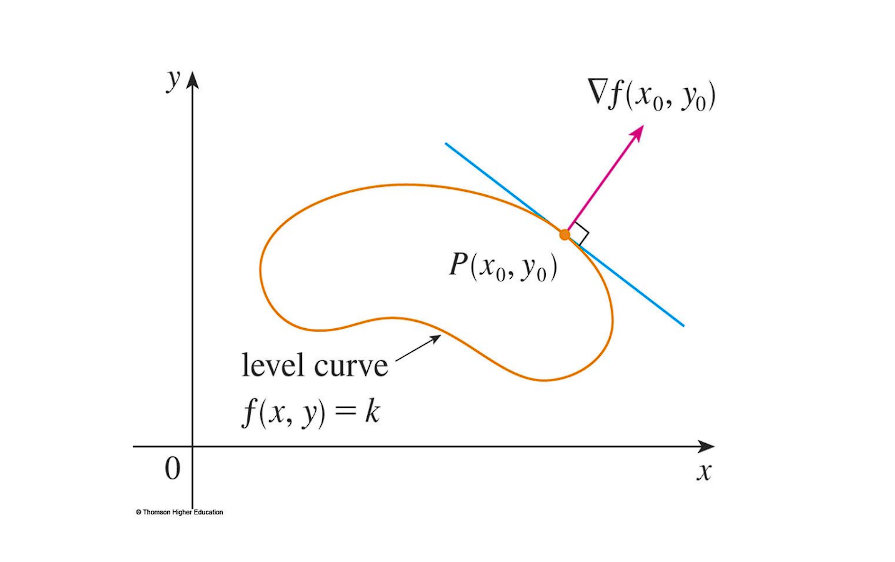
\includegraphics[scale  = 0.5]{8.png}
\end{center}

\begin{mybox}
    Tangent line to a level curve: 
    $$f_x(x_o,y_o)(x -x_o) +f_y(x_o,y_o)(y-y_o) = 0$$
\end{mybox}
Example: Given function $f(x,y) = 3x^2 + 4xy^2$, find equation of tangent line at point $P_o(-1,1)$\\
Sol:\\
$$f_x = 6x + 4y^2$$
$$f_y = 8xy$$
The gradient vector is:$$ \nabla = (6x +4y^2, 8xy)$$
$$\nabla P_o = (-2, -8)$$
Equation of tangent line at $P_o$ on the level curve:
$$-2( x - x_o)+ -8(y - y_o) = 0$$
$$\Leftrightarrow -2(x +1) -8(y -1) = 0$$
$$\Leftrightarrow -2x -2 -8y + 8 = 0$$
$$\Leftrightarrow y = \frac{-1}{4} x + \frac{3}{4}$$
\subsection{Gradient vector perpendicular to level surface}
\begin{mybox}
    Consider a 3 variables function $F(x,y,z)$ and the level surface S is defined by $F(x,y,z) = k$. Suppose $P_o(x_o,y_o,z_o)$ is a point on S. \\
    Then the gradient vector $\nabla F(P_o)$ is orthogonal ( perpendicular) to the tangent of the level surface at $P_o$
\end{mybox}

Equation of tangent plane to the level surface at point $P_o(x_o,y_o,z_o)$ and normal vector $\nabla F(x_o,y_o,z_o)$:
$$\nabla F(x_o,y_o,z_o)(x-x_o,y-y_o,z-z_o) = 0$$
or: 
$$F_x(x_o,y_o,z_o)(x-x_o)+F_y(x_o,y_o,z_o)(y-y_o)+F_z(x_o,y_o,z_o)(z-z_o) = 0$$
\begin{center}
    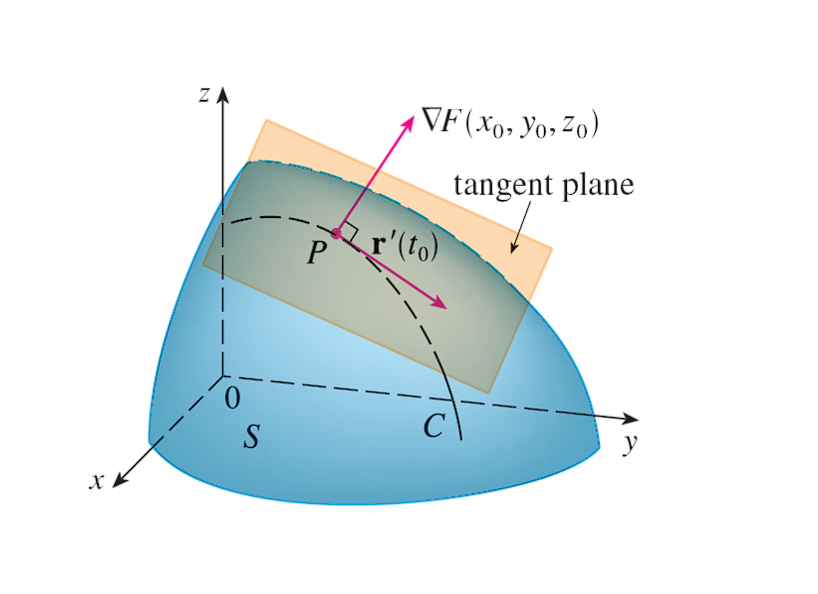
\includegraphics[scale  = 0.5]{9.png}
\end{center}

$\bullet$ Normal line to the surface $F(x,y,z) =k$ at point $P_o(x_o,y_o,z_o)$ can be represented by vector equation: 
$$r = (x_o,y_o,z_o)+ t\nabla F(x_o,y_o,z_o)$$
or:
$$x = x_o +tF_x(x_o,y_o,z_o)$$
$$y = y_o +tF_y(x_o,y_o,z_o)$$
$$z = z_o +tF_z(x_o,y_o,z_o)$$
Example: Find the tangent plane and normal line of the level surface 
$$f(x,y,z) = x^2 +y^2 +z - 9 = 0 $$
at point P(1,2,4)
 \begin{center}
     \textbf{Solution} 
 \end{center}
 \begin{center}
     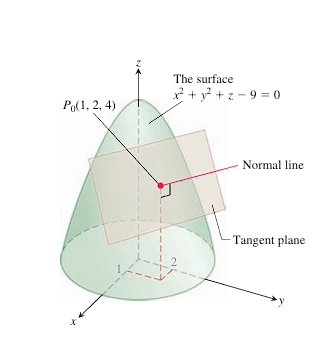
\includegraphics[scale = 0.7]{10.png}
 \end{center}

$\nabla f(P) = (f_x,f_y,f_z) = (2,4,1)$\\
The equation of tangent plane: 
$$ 2(x-1) + 4(y - 2)+ 1(z-4) = 0$$
or 
$$ 2x + 4y + z = 14.$$
Normal line: x = 1 +2t , y = 2 + 4t   , z =4 + t
\subsection{Tangent plane to z =$f(x,y)$ }
\begin{mybox}
    Let $f(x,y)$ be a function of two variables. The equation of the tangent plane to the graph $z = f(x,y)$ at point $(x_o, y_o, f(x_o,y_o))$ given by:
    $$z = f(x_o,y_o) + \nabla f(x_o,y_o)(x-x_o,y-y_o)$$
    or $$z = f(x_o,y_o) + f_x(x_o,y_o)(x-x_o)+f_y(x_o,y_o)(y-y_o)$$
\end{mybox}
\begin{center}
    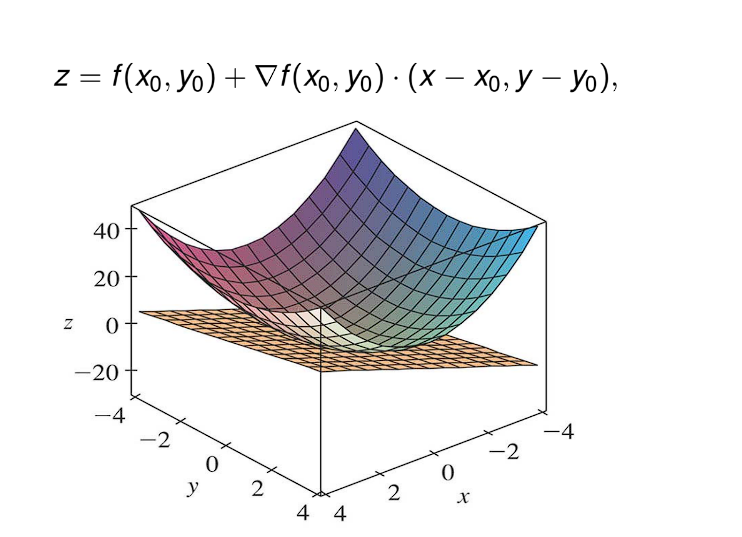
\includegraphics[scale  = 0.5]{11.png}
\end{center}

Example: Find the plane tangent to the surface $z = f(x,y) = xcosy - ye^x$ at point (0,0)
 \begin{center}
     \textbf{Solution} 
 \end{center}
$$f_x = cosy - ye^x$$
$$f_y = -xsiny - e^x$$
Equation of tangent surface is:
$$f(0,0) + f_x(0,0)(x-0) +f_y(0,0)(y-0) = z$$
$$\Leftrightarrow x - y - z = 0$$

\subsection{Linear Approximation of $f(x,y)$ }
The equation of tangent plane to z = f(x, y) at (a, b) is
$$z = f(a,b) + f_x(a,b)(x-a)+f_y(a,b)(y-b)$$
$$Let:  L(x,y) = f(a,b) + f_x(a,b)(x-a)+f_y(a,b)(y-b)$$
\begin{mybox}
    For (x,y) close to (a,b), we use L(x,y) to approximate f(x,y) as follow: 
    $$f(x,y) \approx L(x,y)$$
    that is : 
    $$f(x,y) \approx f(a,b) + \nabla f(a,b)(x-a,y-b) $$
    or:
    $$f(x,y) \approx f(a,b) + f_x(a,b)(x-a)+f_y(a,b)(y-b)$$
\end{mybox}
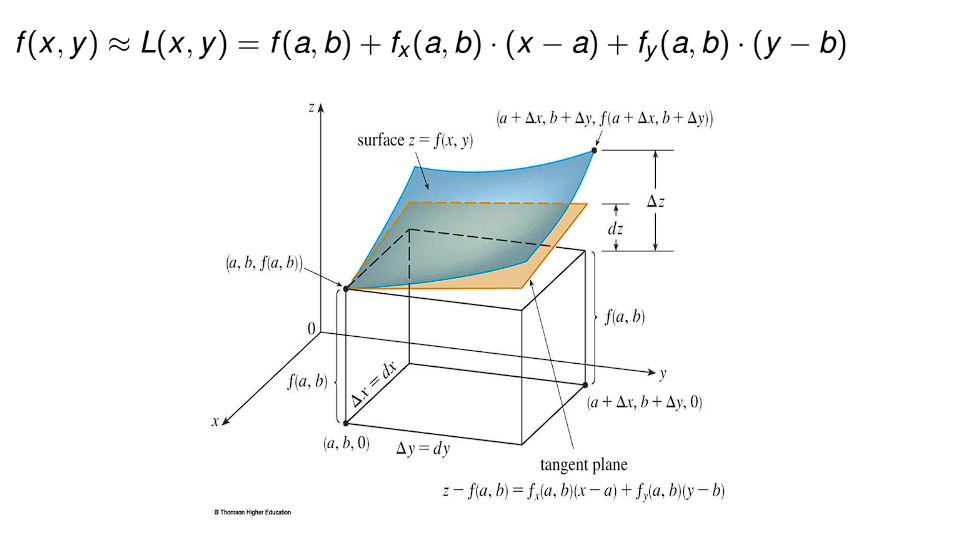
\includegraphics[scale  =0.65]{12.png}\\
Example: Use linear approximation to approximate the value
$$10\times 9.9^2 + 8 \times 6.1^2$$
 \begin{center}
     \textbf{Solution} 
 \end{center}
Choose $f(x,y)=10x^2 +8y^2$ and (a,b) = (10,6) \\
$$f_x(x,y) = 20x$$
$$f_y(x,y) = 16y$$
Using linear approximation, we have:
$$f(9.9,6.1) = f(10,6) + f_x(10,6)(9.9 -10) +f_y(10,6)(6.1-6) = 1277.6$$
\subsection{Estimate change in $f$: Differential }
 The change in f from a point (a, b) to ( a+$\Delta x$,b +$\Delta y$):
 $$\Delta f = f(a+\Delta x,b +\Delta y) - f(a,b)$$
 $$ \rightarrow \Delta f \approx L(a+\Delta x,b +\Delta y) - f(a,b)$$
  $$ \rightarrow \Delta f \approx f_x(a,b)(\Delta x)+f_y(a,b)(\Delta y) $$
 $\Delta x$, $\Delta y$ are small changes in x and y.\\
 $\bullet$ Total Differential
\begin{mybox}
    We define the total differential of f (or simply, the differential of $f$), denoted by $df$, as:
    $$df = \nabla f(a,b) (\Delta x,\Delta y) = f_x(a,b)(\Delta x)+f_y(a,b)(\Delta y) $$
\end{mybox}
Thus, we have : $df \approx \Delta f $\\
Notation is often used: $dx = \Delta x$ and $dy = \Delta y$, so that:\\
$$ df =  f_x(a,b)( dx)+f_y(a,b)(dy)$$
Example: Let $f(x,y) = 6x^5 + 2y^3 $. If x change from 3 to 3.05, y change from 5 to 4.5. Compute $df$
 \begin{center}
     \textbf{Solution} 
 \end{center}
Since x change from 3 to 3.5, y change from 5 to 4.95, we have: 
$$a = 3 \rightarrow \Delta x = 0.05$$
$$b = 5 \rightarrow \Delta y = -0.05$$
And: 
$$f_x = 30x^4 $$
$$f_y = 6y^2$$
$$df = f_x(3,5)\Delta x +f_y(3,5) \Delta y = 114$$
\
$\bullet$ General Case:
\begin{mybox}
    For a function $f(x_1, x_2, x_3,..,x_n)$ of three variables, we have the following linear approximation and total differential at $(a_1, a_2,.., a_n)$ as follows.\\
    \\
    $\bullet$ Linear approximation: \\
    $f(x_1, x_2, x_3,..,x_n) \approx L(x_1, x_2, x_3,..,x_n)$
    $$                        = f(a_1, a_2,.., a_n)+ \nabla  f(a_1, a_2,.., a_n)(x_1-a_1,x_2-a_2,..,x_n -a_n)  $$
    $\bullet$ Total differential:
    $$df = \nabla  f(a_1, a_2,.., a_n)(x_1-a_1,x_2-a_2,..,x_n -a_n) $$
\end{mybox}
    \newpage
\begin{center}
    \textbf{FEEDBACK FOR THIS DOCUMENT}\\
    
\includegraphics[width=0.5\linewidth]{qr.jpg}\\
    \textbf{Please scan this QR code...}\\
    \textbf{Or click this link:} \url{https://forms.gle/qmMhmKmVWHVKNAaG6} \\
    to give us feedback on this document!!!
\end{center}
Please spend a little time to send your feedback. Although it is just a simple work, it has great significance to us. Your feedback can help us improve our future documents and it let us know whether you understand what we have written in this document. Thank you so much for using our documents!\\
\begin{center}
    Good luck with your exam!
\end{center}

\end{document}
